%%%%%%%%%%%%%%%%%%%%%%%%%%%%%%%%%%%%%%%%%%%%%%%%%%%%%%%%%%%%%%%%%%%%%%%%%%%%%%

\chapter{FUNDAMENTAÇÃO}
\label{ch:fun}

{\color{red}
Este capítulo apresenta os conceitos fundamentais relacionados a essa proposta, começando pelo básico de operação dos satélites, apresentando os conceito de \textit{Data Warehouse}, \textit{OLAP} e Cubo de Dados, e por fim a definição de \textit{Big Data} utilizada no trabalho.
}

\section{Operação de Satélites}
\label{ch:fun:operations}

The main characteristic of satellite telemetry data is its high dimensionality in the form of having many telemetries for a given time frame, thus making it a time series.

Telemetry data is measured across all the equipments of the satellite, which can measure widly different values like battery voltage, magnetometer influences and payload healthchecks among others, and is therefore highly complex in nature.
Some satellites can have thousands of telemetries, with some being received per second continuously during its lifetime, like the Hubble telescope that generated terabytes of telemetry data per year [@miebachHubbleSpaceTelescope1998].

Telemetry data

Telemetry data is obtained from the satellites via telecommunication with the ground stations.
For SCC, the data is delivered as raw binary data, which is then converted to a human readable format by SATellite Control System (SATCS), a software system developed by the Ground Systems Development Division (DSS) of coordination of Space Engineering and Technology at INPE [@JulioFoAmbrFerrLour:2017:ChImSp].

SATCS also provides means to send telecommand and some basic data visualization, but these only use recent telemetry data and not the full historical database.
The system is very useful for daily satellite operations, but it lacks the big data analysis that is necessary for a more comprehensive data mining effort, which lead to the proposal of a data mining architecture for telemetry data at INPE [@AzevedoAmbr:2010:ArSaTe].

{\color{red}
\textbf{Dataflow? Explicar a operação de satélites bem por cima}
}

\section{Big Data}
\label{ch:fun:bigdata}

O termo \textit{Big Data} vem evoluindo ao longo dos anos, e para este trabalho vamos utilizar a definição dos \textit{5 Vs}~\cite{bimonteOpenIssuesBig2016}: Volume, Variedade, Velocidade, Valor e Veracidade. Em detalhes:

\begin{itemize}
	\item \textbf{Volume}: esse termo geralmente especifica uma quantidade de dados em que um sistema tradicional de gerenciamento de banco de dados é ineficaz.
É importante ressaltar que isso não se trata apenas do armazenamento dos dados, mas também do seu processamento~\cite{boussoufBigDataBased2018}.
Usar um grande volume de dados geralmente implica em modelos melhores, que então produzem análises melhores, justificando a coleta de uma grande quantidade de dados.
	\item \textbf{Variedade}: dados são provenientes de fontes diferentes, com formatos diferentes, sem um esquema de modelagem padronizado, como dados advindos de \textit{logs} de computadores, dados de sensores, dados multimídia, etc.
Como consequência, esses dados devem ser utilizados da forma mais transparente o possível na análise.
	\item \textbf{Velocidade}: dados são disponibilizados de uma forma muito rápida, e devem ser analisados da forma mais rápida o possível.
Isso implica que os dados podem ser guardados e analisados até em tempo real.
	\item \textbf{Valor}: os dados devem ser armazenados para criar algum valor para os seus usuários, seja ele econômico, científico, social, organizacional, etc.
	\item \textbf{Veracidade}: os dados não possuem garantias quanto a sua qualidade, como inconsistências e falta de acurácia, porém a análise deve ser de alta qualidade de qualquer forma.
\end{itemize}

Estes V's estão relacionados com a construção de um \textit{Data Warehouse}, sendo que também podem ser vistos como requisitos para a crição de um para um conjunto de dados caracterizado como \textit{Big Data}~\cite{zhangBigDataFramework2017}.
Em especial, existe um certo relacionamento com a ideia de "\textit{NoSQL}" ("Não apenas SQL", em inglês), em que não apenas sistemas de banco de dados relacionais são utilizados, mas também outros paradigmas são utilizados, como orientados a documentos, chave e valor, etc~\cite{bimonteOpenIssuesBig2016}.

\section{Data Warehouse}
\label{ch:fun:dw}

Um Armazém de Dados ou Data Warehouse (DW) é um repositório de dados orientado por assunto, integrado, variado ou particionado em função do tempo e não volátil, que auxilia no gerenciamento do processo de tomada decisões~\cite{inmonUsingDataWarehouse1994}.
Essa definição pode ser dividida em:

\begin{itemize}
	\item \textbf{Orientado por assunto}: o DW é utilizado para a análise de uma área em específico.
Por exemplo, é de interesse analisar especialmente os dados da carga útil de uma forma específica.
	\item \textbf{Integrado}: o DW deve integrar dados vindos de múltiplas fontes de uma forma estrutura.
Por exemplo, mesmo que existam duas representações diferentes para um mesmo produto, o DW deve possuir apenas uma representação.
Isso requer o uso de técnicas de limpeza e integração dos dados, de modo a garantir a consistência dos dados.
	\item \textbf{Variado em função do tempo}: o DW deve conter, explícita ou implicitamente a perspectiva de tempo.
Isso quer dizer que o DW possui dados históricos e eles podem ser consultados durante a análise.
Por exemplo, pode se querer saber de dados de dias, meses ou anos atrás.
	\item \textbf{Não volátil}: uma vez dentro do DW, os dados não são removidos ou atualizados, sendo um requisito para a consulta de dados históricos.
\end{itemize}

Essas características diferem o \textit{Data Warehouse} de outros sistemas de repositório, como sistemas de banco de dados, sistemas de processamento de transações e sistemas de arquivos~\cite{hanDataMiningConcepts2011}.

Um DW é geralmente representado por um modelo dimensional que permite eficiência na organização dos dados e na recuperação de informações gerenciais~\cite{kimballDataWarehouseToolkit2013}.
Neste modelo são definidos fatos, dimensões e medidas.
Um fato corresponde ao assunto de negócio a ser analisado, cada dimensão é uma perspectiva de visualização do assunto de negócio e medidas são valores numéricos que quantificam o assunto de negócio.
Uma das dimensões é sempre temporal para permitir a análise do assunto ao longo do tempo~\cite{silva:2015:abordagensParaCubo}.

\section{OLAP}
\label{ch:fun:olap}

\textit{On-line Analytical Processing} (OLAP) é um termo que se refere a um conjunto de ferramentas que são utilizadas para resumir, consolidar, visualizar, aplicar formulações e sintetizar dados de acordo com múltiplas dimensões~\cite{coddProvidingOlapUseranalysts1998}.

Um sistema OLAP permite a resposta de consultas multidimensionais usando dados armazenados no \textit{Data Warehouse}~\cite{kimballDataWarehouseToolkit2013}, sendo que as características principais são~\cite{bimonteOpenIssuesBig2016}:

\begin{itemize}
	\item \textbf{Consultas Online}: as consultas devem ser feitas \textit{Online}, isto é, em tempo real para o usuário.
	\item \textbf{Consultas Multidimensionais}: Consultas são definidas utilizando as dimensões e medidas providas pelo \textit{Data Warehouse}, que esperam dados de alta qualidade.
	\item \textbf{Representação simples}: os resultados das consultas devem ser representados utilizando tabelas e gráficos, pois os usuários finais geralmente são tomadores de decisão que precisam de visualizações relevantes.
	\item \textbf{Exploratórias}: as consultas são utilizadas em carácter exploratório, pois geralmente os usuários não conhecem de antemão todos os dados disponíveis para consultas.
\end{itemize}

Cada ferramenta OLAP deve manipular um novo tipo abstrato de dados (TAD), chamado de cubo de dados, utilizando estratégias específicas devido ao modo de como os dados são armazenados, sendo classificadas em~\cite{moreiraFullPartialData2012}:

\begin{itemize}
	\item \textbf{\textit{Relational OLAP} (ROLAP)}: utilizam Sistemas de Gerenciamento de Banco de Dados (\textit{Data base Management System} - DBMS) relacionais para o gerenciamento e armazenamento dos cubos de dados.
Ferramentas ROLAP incluem otimizações para cada DBMS, implementação da lógica de navegação em agregações, serviços e ferramentas adicionais;
	\item \textbf{\textit{Multidimensional} OLAP (MOLAP)}: implementam estruturas de dados multidimensionais para armazenar cubo de dados em memória principal ou em memória externa.
Não há utilização de repositórios relacionais para armazenar dados multidimensionais e a lógica de navegação já é integrada a estrutura proposta;
	\item \textbf{\textit{Hybrid} OLAP (HOLAP)}: combinam técnicas ROLAP e MOLAP, onde normalmente os dados detalhados são armazenados em base de dados relacionais (ROLAP), e as agregações são armazenadas em estruturas de dados multidimensionais (MOLAP).
\end{itemize}

Além desses, existem sistemas OLAP voltados para um domínio ou estilo de dados específico, como é o caso do \textit{Spatial OLAP} (SOLAP), voltado para consultas espaciais~\cite{viswanathanUsercentricSpatialData2014}.

É importante ressaltar a diferença entre OLAP e \textit{Online Transaction Processing} (OLPT), visto que sistemas comuns de banco de dados utilizam apenas OLTP, que tem o objetivo de realizar transações e processar consultas online.
Isso cobre a grande maioria das operações do dia a dia, como controle de estoque, operações bancárias, etc, servindo a diversos usuários de uma organização.
Já o OLAP é utilizado por tomadores de decisão e analistas de dados, sendo voltado para decisões de mais alto nível na organização~\cite{hanDataMiningConcepts2011}.

\section{Cubo de Dados}
\label{ch:fun:cube}

O Cubo de Dados originalmente foi criado como um operador relacional que gera todas as combinações possíveis de seus atributos de acordo com uma medida~\cite{grayDataCubeRelational1996}.

A estrutura do cubo de dados permite que os dados sejam modelados e visualizados em múltiplas dimensões, e ele é caracterizado por dimensões e medidas.
Uma medida é um atributo cujos valores são calculados pelo relacionamento entre as dimensões, sendo que esse é calculado utilizando funções de agragação como soma, quantidade, média, moda, mediana, etc.
Uma dimensão é feita pelas entidades que compõe os nossos dados, determinando o contexto do assunto em questão~\cite{hanDataMiningConcepts2011}.
Uma dimensão pode ainda ser dividida em membros, que podem ter uma hierarquia, como uma divisão da dimensão tempo em dia, mês e ano.

A organização de um cubo de dados possibilita ao usuário a flexibilidade de visualização dos dados a partir de diferentes perspectivas, já que o operador gera combinações através do conceito do valor \textit{ALL}, onde este conceito representa a agregação de todas as combinações possíveis de um conjunto de valores de atributos.
Operações em cubos de dados existem a fim de materializar estas diferentes visões, permitindo busca e análise interativa dos dados armazenados~\cite{hanDataMiningConcepts2011}.

Um cubo de dados é composto por células e cada célula possui valores para cada dimensão, incluindo \textit{ALL}, e valores para as medidas.
O valor de uma medida é computado para uma determinada célula utilizando níveis de agregação inferiores para gerar os valores dos níveis de agregação superiores na estratégia \textit{Top-down}, com a ordem inversa sendo a \textit{Bottom-up}.

{\color{red} Traduzir exemplo do rodrigo do curso p/ satélites?!}

\subsection{Células do Cubo de Dados}
\label{ch:fun:cube:cells}

{\color{red} Cubóides?! Imagem to lattice tem que vir aqui também}

Um cubo de dados é composto de vários subcubos, que são todos os possíveis níveis de agregação nas dimensões especificadas.
Subcubos são compostos de células base e células agregadas, sendo uma célular agregada é uma célula que utiliza do valor especial \textit{ALL} ($"*"$) para demonstrar que está agregando valores em uma ou mais dimensões.
Uma célula base não utiliza da notação \textit{ALL}, sendo composta do nível mais baixo de agregação~\cite{limaSEQUENTIALPARALLELAPPROACHES2009}.

Formalmente, supondo um cubo de dados $n$-dimensional, uma célula $a$ de qualquer subcubo é definida por $a = (a_1, a_2, a_3, ..., a_n, medidas)$.
A célula é m-dimensional (de um subcubo com $m$ dimensões), se exatamente $m$, com $(m \leq n)$, valores entre $(a_1, a_2, a_3, ..., a_n)$ não são $"*"$.
Se $m = n$, então $a$ é uma célula base, caso contrário $(m < n)$, ela é uma célula agregada.

{\color{red} exemplo}

Um relacionamento de descendente-ancestral pode existir entre células. 
Em um cubo de dados $n$-dimensional, uma célula $a = (a_1, a_2, a_3, ..., a_n, medidas_a)$ de nível $i$ é um ancestral de uma célula $b = (b_1, b_2, b_3, ..., b_n, medidbs_b)$ de nível $j$, e $b$ é um descendente de $a$, se e somente se $i < j$ e $1 \leq m \leq n$, onde $a_m = b_m$ sempre que $a_m \neq *$.
Em particular, uma célula $a$ é chamada de pai de uma célula $b$, e $b$ de filho de $a$, se e somente se $j = i+1$ e $b$ for um descendente de $a$~\cite{hanDataMiningConcepts2011}.

{\color{red} exemplo}

\subsection{Modelagem dimensional}
\label{ch:fun:cube:dimm}

Existem três esquemas principais para a modelagem dimensional de um cubo de dados: Esquema Estrela (\textit{Star Schema}), Esquema Floco de Neve (\textit{Snowflake Schema}) e Constelação de Fatos (\textit{Fact Constellation Schema}).

O esquema estrela é o mais utilizado, sendo que ele contém uma tabela central chamada de tabela de fatos, onde reside a maior parte dos dados, com um conjunto menor de tabelas, chamadas de tabelas de dimensão, para as outras dimensões.
A figura~\ref{fig:starschema} mostra um exemplo de esquema estrela.

\begin{figure}[!htb]
	\caption{Esquema estrela}\label{fig:starschema}
	\vspace{6mm}
	\begin{center}
		\resizebox{4cm}{!}{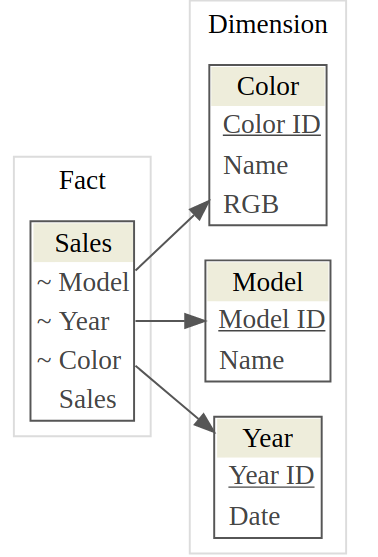
\includegraphics{Figuras/starSchema.png}}
	\end{center}
	\vspace{1mm}
	\legenda{}
	\FONTE{Produção do autor}.
\end{figure}

O esquema floco de neve é uma variação do esquema estrela, onde algumas dimensões são normalizadas, dividindo os dados das tabelas de dimensão em outras tabelas.
Isso possui vantagens de eliminar redundâncias nas tabelas de dimensão, porém cria problemas durante a execução de consultas, visto que é necessário realizar operações de \textit{join} com as novas tabelas.
A figura~\ref{fig:snowflakeschema} mostra um exemplo de esquema floco de neve.

\begin{figure}[!htb]
	\caption{Esquema floco de neve}\label{fig:snowflakeschema}
	\vspace{2mm}
	\begin{center}
		\resizebox{5cm}{!}{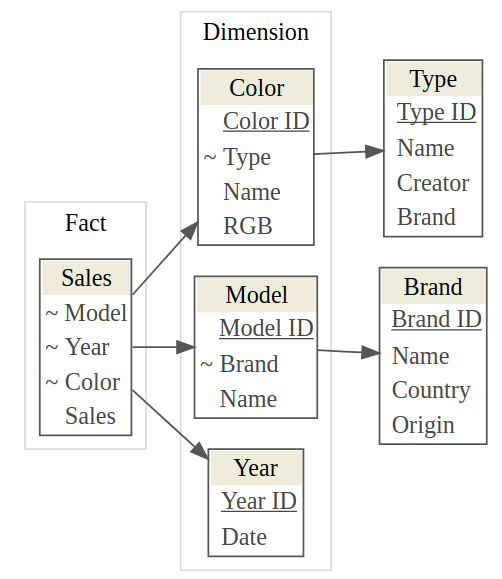
\includegraphics{Figuras/snowflakeSchema.png}}
	\end{center}
	\vspace{1mm}
	\legenda{}
	\FONTE{Produção do autor}.
\end{figure}

O esquema constelação de fatos utiliza de múltiplas tabelas de fato, como se fossem várias tabelas no esquema estrela que compartilham tabelas de dimensão.
Isso leva ao seu nome, como um conjunto de estrelas.
A figura~\ref{fig:factconstschema} mostra um exemplo de constelação de fatos.

\begin{figure}[!htb]
	\caption{Esquema constelação de fatos}\label{fig:factconstschema}
	\vspace{6mm}
	\begin{center}
		\resizebox{7cm}{!}{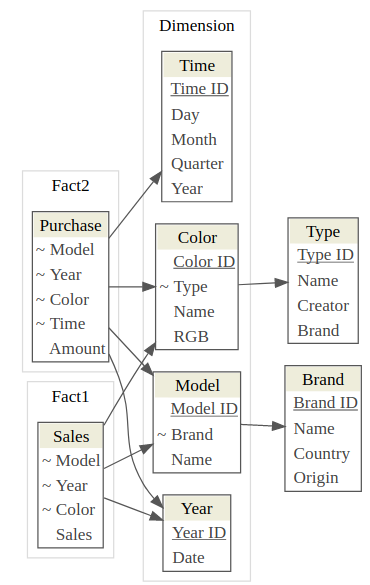
\includegraphics{Figuras/factConstellationSchema.png}}
	\end{center}
	\vspace{2mm}
	\legenda{}
	\FONTE{Produção do autor}.
\end{figure}

\subsection{Hierarquias de conceito}
\label{ch:fun:cube:concept}

Uma hierarquia de conceitos é utilizada para definir uma sequência de mapeamento entre um conjunto de conceitos de baixo nível para um conjunto de conceitos de alto nível, mais gerais.
É um estilo de agrupamento e discretização, pois agrupa os valores de modo a reduzir a cardinalidade de uma dimensão~\cite{hanDataMiningConcepts2011}.
Elas ajudam a tornar a análise mais fácil de ser entendida, pois as operações traduzem os dados de baixo nível em uma representação que é mais fácil para o usuário final, assim facilitando a execução das consultas e o seu subsequente uso.

{\color{red} Han, figura 4.10}

\subsection{Medidas}
\label{ch:fun:cube:measures}

Cada célula de um cubo é definida como um par $\langle (d_1, d_2, ..., d_n), medidas\rangle$, onde $(d_1, d_2, ..., d_n)$ representam as combinações possíveis de valores de atributos sobre as dimensões.
Uma medida é calculada para uma certa célula agregando os dados correspondentes a combinação de dimensões e valores~\cite{hanDataMiningConcepts2011}.
Medidas podem ser classificadas em três tipos: distributiva, algébrica e holística.

Uma medida distributiva é uma medida cujo cálculo pode ser particionado e depois combinado, e o resultado seria o mesmo se o cálculo fosse executado em todo o conjunto de dados.
Por exemplo, a função de soma é distributiva: dividindo os dados $N$ em conjuntos $n$, e fazendo a soma de cada conjunto $n$, teremos o mesmo resultado que se a fosse feita diretamente sobre $N$.

Uma medida algébrica é uma medida cujo cálculo pode ser feito sobre duas ou mais medidas distributivas.
Por exemplo, uma medida de média pode ser calculada com a divisão da medida \textit{soma} pela a medida \textit{contagem}, que são ambas distributivas.

Uma medida é holística se não existe uma medida algébrica com $M$ argumentos que caracterize a computação.
Isso quer dizer que a computação não pode ser particionada, com valores exatos obtidos apenas se a medida for aplicada em todos os dados.
Alguns exemplos são as medidas de moda, desvio padrão e mediana~\cite{hanDataMiningConcepts2011}.

\subsection{Operações OLAP}
\label{ch:fun:cube:olapops}

Para realizar consultas no \textit{Data Warehouse}, é necessário utilizar de algumas operações sobre o cubo de dados para obter os resultados adequados.
Essas consultas também devem conseguir passar na hierarquia de conceitos de cada dimensão, bem como seguir o modelo dimensional do cubo definido, para conseguir oferecer uma interface amigável com o usuário para análise interativa~\cite{hanDataMiningConcepts2011}.
Algumas operações comuns são:

\begin{itemize}
	\item \textit{Roll-up}: realiza agregação no cubo de dados, seja navegando na hierarquia de conceitos de nível específico para um mais genérico, ou reduzindo uma dimensão.
	\item \textit{Drill-down}: o inverso da operação \textit{roll-up}, navega na hierarquia de conceitos do nível mais genérico para o nível mais específico, ou adiciona dimensões ao cubo atual.
Essa operação visa aumentar o nível de detalhes dos dados.
	\item \textit{Slice}: ou "fatiamento", realiza uma seleção em uma dimensão do cubo, resultando em um subcubo.
	\item \textit{Dice}: define um subcubo realizando uma seleção (\textit{slice}) em duas ou mais dimensões.
	\item \textit{Pivot}: também chamada de rotação, permite mudar a posição das dimensões na visualização, portanto alterando linhas por colunas e vice-versa.
\end{itemize}

{\color{red} Rodrigo, figura 2.1}

Dependendo do sistema OLAP, é possível que outras operações sejam possíveis, como \textit{drill-across} que passa por mais do que uma tabela de fatos, e \textit{drill-through} que permite executar consultas direto na representação em baixo nível do cubo~\cite{hanDataMiningConcepts2011}.

\subsection{Computação do cubo de dados}
\label{ch:fun:cube:comp}

A computação do cubo de dados é um problema exponencial em relação ao tempo de execução e ao consumo de memória, portando dada uma relação de entrada \textbf{R} com tuplas de tamanho $n$, a saída é $2^n$, onde $n$ é o número de dimensões de um cubo.

To properly calculate a data cube for some measures and dimensions, you have to count the cardinality of each dimension against the cardinality of all other dimensions.
While manageable for a few dimensions, this computation becomes almost impossible for cubes with high dimensions as the number of combinations becomes too much for a single computer to handle.
This lead to the development of data cube algorithms that optimize for the most relevant measures in the data cube [@silva:2015:abordagensParaCubo].

A *cuboid* is a part of a data cube. For example, if you have three dimensions: temperature, tension and time, a 2-D cuboid could be made from the dimensions temperature and tension, and a 3-D cuboid would be the same as the full data cube, like figure [\@ref(fig:datacube)].
The data cube algorithms focus on the computation of cuboids, as the every cube is composed of these smaller cuboids.
This leads to the existence of the *curse of dimensionality*, as for $n$ of dimensions there will be $2^n$ possible cuboid computations, making full materialization very difficult after a few dimensions [@hanDataMiningConcepts2011;@silva:2015:abordagensParaCubo].

For the algorithms, they can be in three different categories: Computing all the cuboids for the data cube leads to a fully materialized data cube; not computing any cuboid beforehand leads to a non-materialized data cube, and partially computing some cuboids leads to partial materialization.

The non-materialized cube has the lowest amount of required memory, but the highest query response time.
The fully materialized cube leads to the lowest query response times, as all combinations are already computed, but it needs the highest amount of memory and is thus very hard to compute.
As for the partially materialized cube, it is the main issue for most of the algorithms: how to materialize only the most relevant cuboids, and thus achieve a good compromise between memory usage and query performance?

There's some different types of partially materialized cubes, like the *iceberg*, which is a cube with only cells that have passed a certain condition; *shell fragments* compute only cubes with a few dimensions (from 3 to 5) and aggregate those cubes when a bigger number of dimensions is required and *closed cubes* are cubes whose cells with identical measures are grouped into a single abstraction, also called *closed cells*.

To choose which cuboids to materialize, there's a plethora of different algorithms.
Two of the classical ones are *Bottom-up* or *Top-down* strategies.
Bottom-up starts from the most specific cuboid, called the base cuboid, and goes to the less specific cuboid.
Top-down is the inverse: it starts from the least specific cuboid, called the apex cuboid, and goes to the base cuboid.
Most of these are tested and overviewed in [@silva:2015:abordagensParaCubo], and won't be repeated here for brevity.

[BUC, Top-down, Bottom-up]

